\documentclass[12pt]{article}
\usepackage[T1]{fontenc}
\usepackage{jwstproposaltemplate_v6}
\usepackage{graphicx}
\usepackage{xcolor}
% Red markers: numbers or checks still to be computed/verified. Remove before submission.
\newcommand{\calc}[1]{\textcolor{red}{#1}}
\newcommand{\todo}[1]{\textcolor{red}{[#1]}}
\begin{document}
\scientificjustification

\noindent\textbf{Does circumnuclear dust remember an AGN's accretion history?}
Large luminosity changes in quasars and other active galactic nuclei provide timed experiments on circumnuclear dust. The relevant population includes strongly variable quasars [1--4] and changing-look AGN [5]. Existing grains heat or cool as the changed radiation reaches them; grains may also be destroyed or form at new locations. \textbf{Can delayed illumination of a fixed dust distribution explain the infrared spectra through brightening, fading and recovery, or must the emitting distribution evolve?} We use measured luminosity histories to test this question. The answer determines how infrared spectra trace an AGN's power and dust covering factor during variability.

The equilibrium sublimation radius scales approximately as $L^{1/2}$ [6--8], but the emitting distribution need not adjust immediately. Brightening tests whether increased heating suffices or the inner dust changes; after fading, surviving dust cools and newly formed inner dust may restore a hotter component. More distant, warmer-to-cooler dust echoes earlier illumination and retains the longest memory. We propose MIRI/MRS spectroscopy of \calc{N} variable AGN, each of which already has a decade of ZTF and WISE photometry, SDSS and new 2026 Palomar optical spectra, and a multi-epoch SPHEREx near-infrared spectral history \todo{confirm SPHEREx epochs exist for every target}. SPHEREx follows the fast-responding hot dust in time; MRS measures the warm dust that should still echo earlier states. Figure~1 shows P1823 in a high optical state, with a long spectral baseline and a WISE decline followed by recovery.

\noindent\textbf{From infrared variability to dust physics.}
WISE observations establish that the infrared emission echoes changing-look transitions [9--12], and mid-infrared variability alone can select such sources [10,12,13]; see [14] for a review. A change in infrared colour, however, can reflect temperature, emitting area, extinction or host dilution. Individual reverberation studies show why a broader test is needed. In Mrk~590, the inner dust radius became smaller following a luminosity decline, implying replenishment within a few years [15]. In NGC~4151, the hottest dust remained at roughly the same radius over decades, while the warm emission had a much longer response [16]. These results motivate testing contrasting histories, and they single out the warm component as the one that distinguishes an echo from a structural change.

JWST supplies the missing spectral information. MRS spectra reveal substantial diversity beyond current dust models [17], including a distinctive silicate spectrum in the recently activated nucleus Ansky [18]. We test the same physical model against spectra and preceding histories. \textbf{The gain is a constrained comparison of delayed heating and dust evolution across known histories.}

\noindent\textbf{SPHEREx tracks the hot dust; MIRI measures the memory.}
SPHEREx provides 0.75--5~$\mu$m all-sky spectroscopy, repeated every six months [19], so each target has a near-infrared spectral time series of its hot dust; P1823 has three dated epochs (Figure~1), and the sample will have \calc{$\geq$X} epochs per target by Cycle~6. SPHEREx cannot see beyond 5~$\mu$m, where AGN variability is strongly damped: at 24~$\mu$m the amplitude is typically $\lesssim$10\% of that in W1 [20], so the warm dust averages over a longer stretch of the history. Its 6.2$''$ pixels also blend nucleus and host. MIRI/MRS supplies both missing pieces: the warm continuum, silicate features, aromatic bands and ionic lines from 4.9 to 27.9~$\mu$m, with sub-arcsecond resolution in channel~1 that separates the nuclear point source from measurable host emission [21]. The division of labour is physical. A fixed dust distribution must explain the SPHEREx hot-dust history and the MRS warm-dust spectrum with a single geometry.

\noindent\textbf{A prepared sample with measured histories.}
The sample is the product of completed preparatory work, not a catalogue query. We selected targets in a low-dimensional manifold learned from the joint ZTF and WISE light curves of \calc{N$_{\rm parent}$} variable AGN [22] \todo{confirm [22] describes the manifold; otherwise cite the right paper}. The manifold organizes sources by the shape of their optical and infrared histories rather than by amplitude alone, so we choose rising, fading and recovering histories deliberately and know where each target sits within the parent population. Every target has an SDSS spectrum from \calc{YYYY--YYYY} and new Palomar \calc{[instrument]} spectroscopy from 2026 \calc{[N objects; dates]}: the change in continuum and broad-line luminosity is measured spectroscopically, not inferred from photometry. With the 2010 WISE W3/W4 baseline and the SPHEREx epochs, each nucleus enters JWST with a measured illumination history and a dated record of its hot-dust response. \textbf{JWST time is spent only on the one measurement no other facility can make.}
\clearpage
\begin{figure}[!ht]
\centering
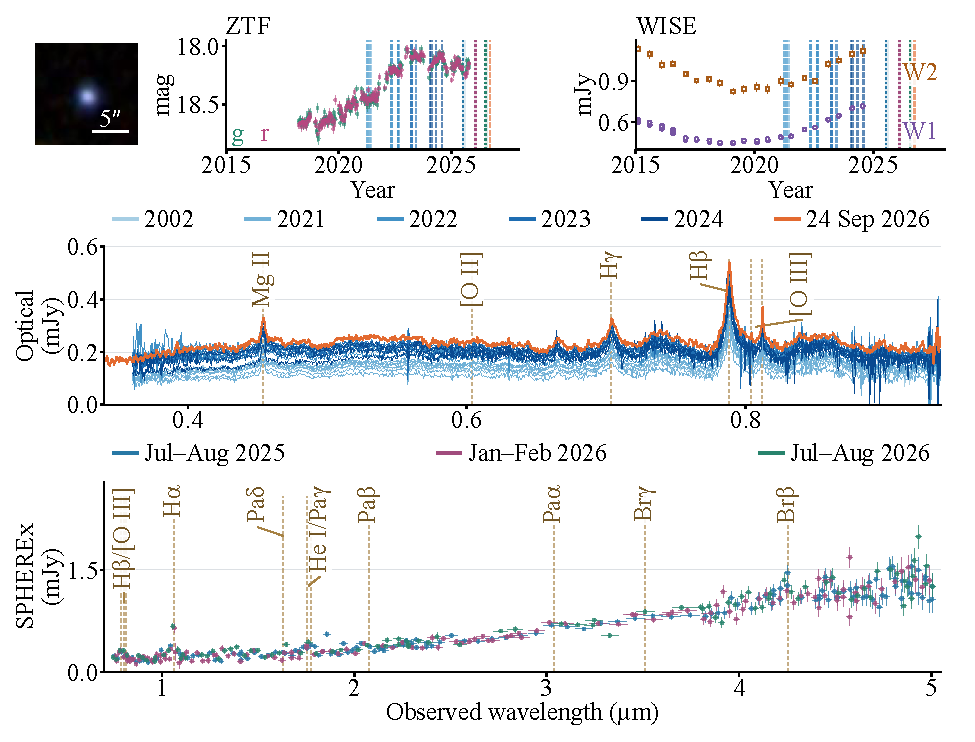
\includegraphics[width=\textwidth]{fig1_connected.pdf}
\caption{\textbf{P1823 connects a measured luminosity history to the infrared spectrum.} The quasar ($z=0.620$) is in a high optical state; WISE records an earlier decline and recovery. Top: SDSS cutout (5$''$ bar), ZTF $g,r$ and WISE W1 (purple circles), W2 (brown squares) histories from 2015. Middle: 21 optical epochs. Bottom: three SPHEREx visits. Date keys above both spectra match the light-curve markers: dashed lines mark optical epochs; dotted lines mark SPHEREx median dates, with shading spanning each visit. The 2002 spectrum predates the displayed time window. Spectral axes use observed $\mu$m and $F_\nu$ in mJy; WISE fluxes are in mJy. Gold markers show expected emission-line positions, not fitted detections.}
\end{figure}

\noindent\textbf{Can changing illumination explain the dust spectrum?}
Figure~1 supplies the optical history and dated near-infrared spectra; MIRI adds the longer-wavelength dust spectrum. We first anchor a fixed dust distribution to the measured luminosity history and the SPHEREx hot-dust epochs, including light-travel delays, host emission and reddening. That model then makes a prediction for the warm continuum and silicate features at the MIRI date. We next allow the amount or location of inner dust to change and test whether the data require that extra freedom. Figure~2 shows that the two scenarios separate by \calc{X~dex} in the warm-dust residual at the achieved precision for \calc{the sample's range of $\Delta t/\tau_{\rm dust}$}. Agreement with fixed dust places limits on structural changes; a persistent, history-dependent mismatch requires dust evolution.

\begin{figure}[!ht]
\centering
\fbox{\parbox{0.9\textwidth}{\centering\vspace{2.5cm}\calc{FIGURE 2 PLACEHOLDER}\vspace{2.5cm}}}
\caption{\calc{\textbf{Fixed and evolving dust make distinguishable predictions.} Predicted warm-dust residual $\delta_{\rm warm}$ versus $\Delta t/\tau_{\rm dust}$ for fixed-distribution and evolving models, for rising, fading and recovering histories. Error bars show expected MRS precision including calibration covariance; markers show each target's position in the Cycle~6 window.}}
\end{figure}

\clearpage
\descriptionofobservations

\noindent\textbf{Targets and wavelength coverage.}
The sample contains \calc{n$_{\rm IR}$} infrared-selected variable candidates [22] and \calc{n$_{\rm CL}$} catalogue CLAGN [23--26], all placed in the ZTF/WISE light-curve manifold and screened for \calc{[criteria: redshift, nuclear W3 flux, host fraction, visibility]}. Table~\calc{X} lists, for every target, the ZTF/WISE baseline, SDSS and Palomar spectral epochs, and SPHEREx epochs. \calc{N$-$1} have $z<0.3$, placing both silicate peaks within MRS; P1823 ($z=0.620$) supplies a well-sampled optical/SPHEREx history and the 9.7~$\mu$m feature at 15.7~$\mu$m. Its 18~$\mu$m peak lies beyond MRS. The primary diagnostics do not depend on channel~4C [21]. Archival total-source W3 and W4 fluxes span approximately \calc{1.4--24} and \calc{3.3--75}~mJy; nuclear fluxes are estimated from \calc{[method]} for exposure design. \todo{P8548: W4 S/N = 2.5; justify retaining or replace}

\noindent\textbf{Selecting histories that test different response times.}
The relevant clock is the rest-frame time since a luminosity change, $\Delta t=(t_{\rm JWST}-t_{\rm change})/(1+z)$, compared with the expected rest-frame delays of the hot and warm dust, $\tau_{\rm dust}$ and $\tau_{\rm warm}$. These depend on luminosity, approximately as $L^{1/2}$ [8,20,27]; equal calendar ages do not imply equal response phases. We bracket changes with optical photometry and spectra, and estimate lag ranges from measured luminosities or reverberation constraints where available. Uncertain event dates, host subtraction and lag scatter enter the comparison. Table~\calc{X} lists $z$, history family, change interval, $\tau_{\rm dust}$, $\tau_{\rm warm}$ and $\Delta t/\tau_{\rm dust}$ at Cycle~6 for every target. \todo{build table}

We prioritize complementary histories: rising sources test prompt heating against the slower warm response; sustained faint states test cooling and possible inner-dust replenishment; recovery tests whether the infrared spectrum depends on earlier illumination as well as current brightness, as in SDSS~J110057.70$-$005304.5, which faded and then recovered over $\approx$20~yr [12]. For a decline followed for several hot-dust delays, a remaining mismatch is harder to attribute to the initial echo alone, while the warm component can still retain an older history [15,16]. Each source is tested against its own dated baseline, with luminosity and host differences included in comparisons between sources.

The saved light curves provide contrasting examples: P1823 brightens over 2019--2023; P11530 fades over 2018--2021 and partly recovers in 2022--2023; P9694 brightens between 2021 and 2022 and remains brighter through 2025. Additional histories include optical decline through 2025, recovery after earlier fading, and a reversal in 2025. The sample spans $\Delta t/\tau_{\rm dust}=\calc{X}$--$\calc{Y}$ and $\Delta t/\tau_{\rm warm}=\calc{X}$--$\calc{Y}$ at Cycle~6; the \calc{K} sources added in this design were selected at \calc{early response phase, $\Delta t/\tau_{\rm dust}\lesssim X$}. Broad-line appearance or disappearance is not required.

\noindent\textbf{Observing at an informative epoch.}
Cycle~6 nominally runs from July 2027 to June 2028 [28]. Selection evaluates each history across the allowed JWST dates, favouring sources whose model comparison remains informative across broad visibility windows rather than depending on catching an unpredictable peak. Contemporary optical coverage connects the saved light curves, mostly ending in 2025, to JWST. Earlier WISE and SPHEREx epochs constrain the preceding hot-dust response; they are fitted at their actual dates and are not assumed to represent the JWST state.

\noindent\textbf{Why \calc{N} sources?}
The sample places \calc{n$_{\rm R}$}, \calc{n$_{\rm F}$} and \calc{n$_{\rm C}$} sources in the rising, fading and recovering families, to distinguish recurring behaviour from individual peculiarities. The within-family scatter in the warm-dust residual, estimated from existing MRS AGN spectra [17], is $s\approx\calc{X}$~dex. Family means then reach \calc{$s/\sqrt{n}$ = X}~dex and rising--fading differences \calc{$s\sqrt{2/n}$ = X}~dex, compared with a predicted history effect of \calc{Y}~dex (Figure~2). Because each source also carries its own SPHEREx time series, it serves as its own control; the ensemble tests replication. We test sensitivity to individual objects and include unequal errors, intrinsic scatter and shared model uncertainties. Inference concerns this deliberately selected sample; population-wide rates would require a selection function.

\clearpage
\noindent\textbf{MIRI/MRS.}
One visit per target uses all three grating settings, target acquisition and a four-point dither, covering approximately 4.9--27.9~$\mu$m [21,29]. We use \calc{FASTR1} readout. Dedicated sky observations are taken for the \calc{M} targets with extended host emission in the MRS field; point-source-dominated nuclei use dither-pair background subtraction [29]. Exposure design is driven by the nuclear continuum and the 18~$\mu$m feature, reaching S/N $\geq$\calc{50} per $R=100$ continuum bin near rest 5 and 12~$\mu$m and $\geq$\calc{30} across the longer-wavelength feature, based on ETC calculations with conservative nuclear spectra and host backgrounds. \todo{ETC per target}

\noindent\textbf{Near-infrared and optical state.}
No near-infrared JWST observations are requested. SPHEREx survey coverage \todo{confirm operations through 2027--28} places a near-infrared spectral epoch within about three months of each MIRI visit without an imposed timing constraint; actual dates enter the fit. The short overlap near 4.9--5.0~$\mu$m provides a check on the relative aperture and host correction between SPHEREx and MRS. Optical spectroscopy near each MIRI visit continues our Palomar program \todo{confirm continuation through 2027--28}, extending each spectral history to the JWST epoch; broad Pa$\alpha$ from \calc{[facility]} constrains the nuclear state and reddening; for $z\lesssim\calc{0.05}$, where Pa$\alpha$ falls in strong telluric absorption, we use \calc{Pa$\beta$ and Br$\gamma$}. One MIRI epoch tests each source against its preceding history; repeat epochs would require a predicted detectable change over an accessible interval and are not requested.

\noindent\textbf{Resources and feasibility.}
The program requests \textbf{\calc{X}~h} for \calc{N} MRS visits, including dedicated sky where required, a Medium program under the Cycle~6 limits [28]. \todo{confirm total within Cycle 6 Medium threshold} Totals come from APT using the ETC exposure times above. Wavelength-dependent calibration errors enter separately from statistical noise [30].

\clearpage
\noindent\textbf{Using the archival baseline correctly.}
The 2010 W3/W4 fluxes constrain earlier emission in large apertures. We predict them by integrating redshifted nuclear-plus-host models through the WISE bandpasses, including colour corrections and uncertainty beyond MRS coverage. Archival imaging constrains host light outside the MRS field; an uncertain nuclear baseline becomes an interval or upper bound. Each target has its own host and aperture model, checked against imaging and spatially resolved host emission where measurable.

\noindent\textbf{Joint spectral and temporal inference.}
We will decompose each cube into a point source and extended emission [17], then jointly fit continuum, silicates, aromatic bands, H$_2$ and ionic lines [31]. Aromatic bands and [Ne\,\textsc{ii}] constrain host contamination; [Ne\,\textsc{v}] and [Ne\,\textsc{vi}] measurements or limits constrain the hard ionizing component. The torus remains spatially unresolved. Optical decomposition constrains the illumination history; the SDSS and 2026 Palomar spectra calibrate the photometric light curves to continuum and broad-line luminosity at their dates, and we marginalize over unobserved intervals and the conversion to heating luminosity. WISE photometry and SPHEREx spectra are fitted as reprocessed emission at their actual dates, with the SPHEREx aperture modelled against the host decomposition.

The fixed-distribution model varies illumination with retarded time while keeping geometry and grain properties constant, spanning clumpy and disk-plus-wind geometries [32--34]. The evolving model allows the inner emitting distribution to change while treating illumination, extinction and host emission in the same way. Anchoring both to the SPHEREx hot-dust epochs limits the geometric freedom before the MRS spectrum is compared. Silicate absorption alone is not a unique test of obscuration. Model comparisons include wavelength-dependent calibration covariance and alternative host decompositions; simulated observations establish which changes are distinguishable at the achieved precision (Figure~2). Residuals shared across the sample indicate shortcomings in the model family. Residuals associated with luminosity history motivate additional dust evolution.

\noindent\textbf{A common diagnostic across histories.}
The primary ensemble diagnostic is $\delta_{\rm warm}$, the logarithmic residual of the rest 8--13~$\mu$m warm-dust continuum luminosity measured by MRS relative to the fixed-distribution prediction, where that prediction is anchored to the optical history and the SPHEREx hot-dust epochs. The decomposition separates dust from direct continuum, lines and host light. As a secondary diagnostic we report the hot-to-warm ratio (rest 2--5 to 8--13~$\mu$m), with the hot component taken from the model-interpolated SPHEREx history at the MIRI date. We compare rising and fading histories first, with recovery as a secondary comparison, and model $\delta_{\rm warm}$ against continuous $\Delta t/\tau_{\rm dust}$ and $\Delta t/\tau_{\rm warm}$. Class labels do not replace the full illumination history. Luminosity and host contribution enter as covariates; source-by-source fits and removal of individual objects test whether an ensemble result is driven by one unusual nucleus.

\clearpage
\supplementalinformation
\noindent\textbf{Special requirements.} None. No timing constraints are requested; exact dates and intervening variability enter the modelling. \todo{confirm no source needs a narrower window [28]} Visibility and schedulability have been checked in APT. \todo{APT check} No coordinated parallels or joint-facility time are requested. Supporting optical spectroscopy continues through our Palomar program \calc{[program ID/semesters]}; near-infrared spectroscopy through \calc{[program]}.

\noindent\textbf{Duplications.} \todo{Target-by-target archive and APT duplication check, including approved observations.} Archival infrared spectra, where available, will be included at their original dates and apertures.

\references
\noindent [1] Rumbaugh, N., et al. 2018, ApJ, 854, 160.\par
\noindent [2] Graham, M. J., Djorgovski, S. G., Drake, A. J., et al. 2017, MNRAS, 470, 4112.\par
\noindent [3] MacLeod, C. L., et al. 2019, ApJ, 874, 8.\par
\noindent [4] Graham, M. J., Ross, N. P., Stern, D., et al. 2020, MNRAS, 491, 4925.\par
\noindent [5] Ricci, C., \& Trakhtenbrot, B. 2023, Nature Astronomy, 7, 1282.\par
\noindent [6] Barvainis, R. 1987, ApJ, 320, 537.\par
\noindent [7] Kishimoto, M., H\"onig, S. F., Beckert, T., \& Weigelt, G. 2007, A\&A, 476, 713.\par
\noindent [8] Koshida, S., et al. 2014, ApJ, 788, 159.\par
\noindent [9] Sheng, Z., et al. 2017, ApJL, 846, L7.\par
\noindent [10] Stern, D., et al. 2018, ApJ, 864, 27.\par
\noindent [11] Yang, Q., et al. 2018, ApJ, 862, 109.\par
\noindent [12] Ross, N. P., Ford, K. E. S., Graham, M., et al. 2018, MNRAS, 480, 4468.\par
\noindent [13] Assef, R. J., Stern, D., Noirot, G., et al. 2018, ApJS, 234, 23.\par
\noindent [14] Lyu, J., \& Rieke, G. 2022, Universe, 8, 304.\par
\noindent [15] Kokubo, M., \& Minezaki, T. 2020, MNRAS, 491, 4615.\par
\noindent [16] Lyu, J., \& Rieke, G. H. 2021, ApJ, 912, 126.\par
\noindent [17] Gonz\'alez-Mart\'in, O., et al. 2025, MNRAS, 539, 2158.\par
\noindent [18] S\'anchez-S\'aez, P., et al. 2026, arXiv:2607.00921.\par
\noindent [19] IPAC/IRSA, ``SPHEREx Data Explorer: Overview'', accessed 2026 September 26.\par
\noindent [20] Lyu, J., Rieke, G. H., \& Smith, P. S. 2019, ApJ, 886, 33.\par
\noindent [21] STScI, JWST User Documentation, ``MIRI Medium Resolution Spectroscopy'', accessed 2026 September 25--26.\par
\noindent [22] Hemmati, S., et al. 2026, ApJ, 998, 130.\par
\noindent [23] Panda, S., \& \'Sniegowska, M. 2024, ApJS, 272, 13.\par
\noindent [24] Zeltyn, G., et al. 2024, ApJ, 966, 85.\par
\noindent [25] Guo, W.-J., et al. 2025, ApJS, 278, 28.\par
\noindent [26] Dong, Q., et al. 2025, ApJ, 986, 160.\par
\noindent [27] Minezaki, T., et al. 2019, arXiv:1910.08722.\par
\noindent [28] STScI, ``JWST Call for Proposals for Cycle 6'' and ``JWST Observations Needing Special Requirements'', accessed 2026 September 26.\par
\noindent [29] STScI, JWST User Documentation, ``MIRI MRS Recommended Strategies'' and ``MIRI MRS Dedicated Sky Observations'', accessed 2026 September 25--26.\par
\noindent [30] STScI, JWST User Documentation, ``MIRI MRS Calibration Status'', accessed 2026 September 25--26.\par
\noindent [31] Donnan, F. R., et al. 2023, MNRAS, 519, 3691.\par
\noindent [32] Nenkova, M., et al. 2008, ApJ, 685, 160.\par
\noindent [33] H\"onig, S. F., Kishimoto, M., Tristram, K. R. W., et al. 2013, ApJ, 771, 87.\par
\noindent [34] H\"onig, S. F., \& Kishimoto, M. 2017, ApJL, 838, L20.\par

\end{document}
